\newcommand{\auteur}{Stalder Lawrence, Pombo Dias Miguel, Cotza Andrea Roberto, \\
	
	Verdasca Jimmy, Clavier Tony \& Guillod Maxime}
\newcommand{\cours}{GEN}
\newcommand{\ecole}{IL --- TIC --- HEIG-VD}
\newcommand{\domaine}{PDG}
\newcommand{\titre}{WordOn Desktop}

\documentclass[a4paper,12pt]{article}
%
\author{\auteur}
\title{\titre}
\date{\today}

\usepackage[frenchb]{babel}
\usepackage{fancyhdr}
\usepackage{graphicx}
\usepackage{amsmath}
\usepackage{listingsutf8}
\usepackage{color}
\usepackage{enumerate}
\usepackage[utf8]{inputenc}
\usepackage[T1]{fontenc}
\usepackage{float}
\usepackage{geometry}
\usepackage{amssymb,mathtools,pifont}
\usepackage{enumitem}
\usepackage{xspace}
\usepackage{appendix}
\usepackage{pdfpages}
% Liens
\usepackage[hyphens]{url}
\usepackage{hyperref}
\geometry{verbose,tmargin=2.5cm,bmargin=2.8cm,lmargin=1.8cm,rmargin=1.8cm}
\selectlanguage{frenchb}
\frenchbsetup{StandardLists=true}
\DeclareGraphicsExtensions{.pdf,.png,.jpg}
\setlength\parindent{0pt}
\setlength{\parskip}{0.7em}

\usepackage{listings}
\lstset{
	breaklines=true, 
	basicstyle=\scriptsize,
	inputencoding=utf8/latin1,
	extendedchars=true,
	numbers=left,
	firstnumber=1,
	numberfirstline=true, 
	language=Java,
	keywordstyle=\color{blue}\ttfamily,
	stringstyle=\color{red}\ttfamily,
	commentstyle=\color{black}\ttfamily
}


% headers & footers
\pagestyle{fancy}

\lhead{\domaine}
\rhead{\titre\space
\includegraphics[scale=0.12]{logo/logo.png}}

\renewcommand{\footrulewidth}{0.4pt}% default is 0pt
\lfoot{\auteur}
\cfoot{}
\rfoot{\thepage}

%%%%%%%%%%%%%%%%%%%%%%%%%%%%%%%%%%%%%%%
%%%%%%% BEGIN DOCUMENT
%%%%%%%%%%%%%%%%%%%%%%%%%%%%%%%%%%%%%%%

\begin{document}
	\clearpage
	\maketitle
	\thispagestyle{empty}
	
	\maketitle
	\begin{figure}[h!]
		\centering
		
\includegraphics[scale=1]{logo/logo.png}
	\end{figure}
	\newpage
	
	% % Entete première page
	% \thispagestyle{empty}
	% %
	% \noindent \cours \hfill \ecole{} \newline
	% \noindent \auteur \hfill \today \newline
	% \hrule
	% \vspace{7mm}
	% \noindent {\large \bf \domaine } \hfill \titre {\large \bf }\\[3mm]
	% \hrule
	
	\tableofcontents
	
	\listoffigures
	
	% On a pas de tableau
	% \listoftables
	
	\newpage
	
	\section{Description générale du projet}
	\subsection{Cadre / contexte}
	Ce projet a lieu dans le cadre du cours PDG à la HEIG-VD à Yverdon-les-Bains dans le cadre de notre dernière année de bachelor en informatique.
	
	\subsection{But(s) visé(s)}
	A l'issue de ce cours ainsi que de ce projet, nous devrons être capables de spécifier, coder ainsi que tester une application de taille importante.
	
	De plus, ce projet nous apprend à acquérir par nous-mêmes des connaissances sur des nouveaux sujets en fonction de nos besoins lors de la création de notre application. 
	
	Il y a également toute la gestion de la problématique d'un projet en équipe, en groupe de 6 personnes. En effet, ceci demande une très bonne coordination entre chaque membre afin de bien séparer le travail et de faire en sorte d'avoir un projet unique et harmonieux à terme. Ceci nous demandera d'utiliser plusieurs outils spécifiques.
	
	\section{Description du jeu sur Smartphone}
		\subsection{Fonctionnalités offertes}
			\subsubsection{Inscription}
			
			\subsubsection{Mode normal}
			\subsubsection{Mode tournoi}
			\subsubsection{Bonus}
		
		\subsection{Règles du jeu}
			\subsubsection{Mode tournoi}
	
	\section{Jeu sur PC}
	\subsection{Introduction}
	Nous avons du optimiser principalement l'interface afin de correspondre aux spécifications d'un ordinateur.\\
	Pour la partie logique, nous avons essayé de coller au mieux à l'application afin de pouvoir offrir une expérince utilisateurs similaire que sur la version mobile. 
	
	\subsection{Structure du projet}
	Nous avons 	séparer notre projet en trois sous-projets afin de faciliter la programmation.  \\
	On utilise Maven pour lier et gérer les dépendances entres ces sous-projets.
	
		\subsubsection{Client}
		Ce sous-projet contient toute la partie pour le client, en d'autres therme pour l'utilisateur. Il contient également toutes les ressources graphique utilisées pour l'affichages, telles que les tuiles, le logo, et tout les boutons.
		
		\subsubsection{Server}
		Celui-ci contient tout le code côté serveur avec toute la logique que cella implique. \\
		C'est lui qui va gérer toute les communications avec tout les clients possibles, mais également de l'intégrité de chaque partie, de générer les bons stacks de lettre en fonction de notre dictionnaire, de verifier les mots envoyés par les clients et en cas de succès, d'envoyer aux 2 joueurs les retours correspondants, etc.
		
		\subsubsection{Common}
		Ce dernier sous-projet contient toutes les classes communes au client ainsi qu'au serveur \textit{Server}. Toutes les classes pouvant passer par le réseau pour communiquer entre le serveur et un client doit donc s'y trouver. \\
		Cette façon de séparer les parties communes nous permet d'éviter le dublicat de code et de s'assurer que les deux autres sous-projets incluent le sous-proket \textit{common} afin de garantir que nos classes comunes le restent.
	
	
	\subsection{Interface graphique}
	L'interface utilisateur à été revue et optimisée pour l'affichage sur ordinateur en raison de la taille d'écran ainsi que sa résolution plus importante. \\
	Cependant, nous avons voulu garder la patte graphique du jeu original sur mobile en reprenant les codes couleurs et les éléments visuels spécifique au jeu.
	
		\subsubsection{Connexion et inscription}
		Les fenêtres de connexion (\textit{SignIn}) ainsi que celle de l'enregistrement (\textit{SignUp}) sont épurée afin de n'afficher que les informations utiles.
		
		\begin{figure}[h]
			\centering
			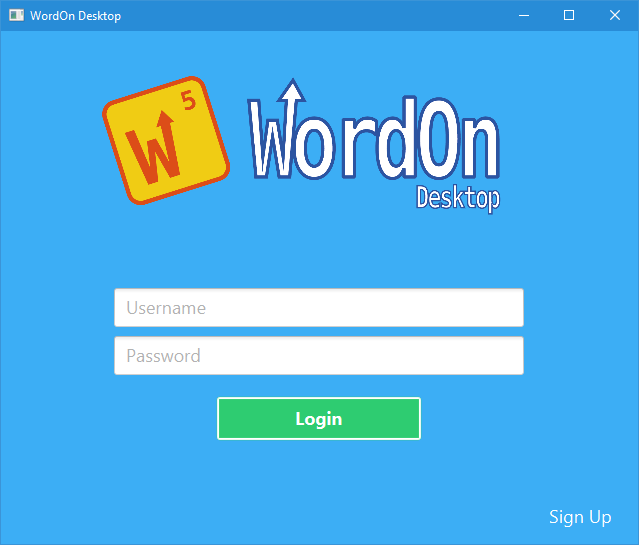
\includegraphics[width=0.4\linewidth]{img/signin.jpg}
			\caption{Fenêtre de connexion}
		\end{figure}
	
		\begin{figure}[h]
			\centering
			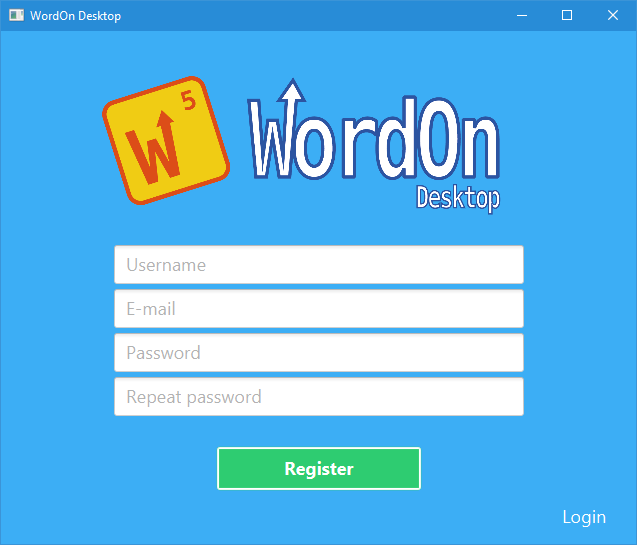
\includegraphics[width=0.4\linewidth]{img/signup.jpg}
			\caption{Fenêtre d'enregistrement}
		\end{figure}
		
		\subsubsection{Jeu}
		La taille plus importante de l'écran nous permet nottament d'afficher le lobby, la partie séléctionnée ainsi que le chat correspondant à la partie en cours. Ceci rend l'expérience de jeu plus adaptée à l'environnement desktop et permet une meilleure vue de toutes les parties en cours.
		
		\begin{figure}[h]
			\centering
			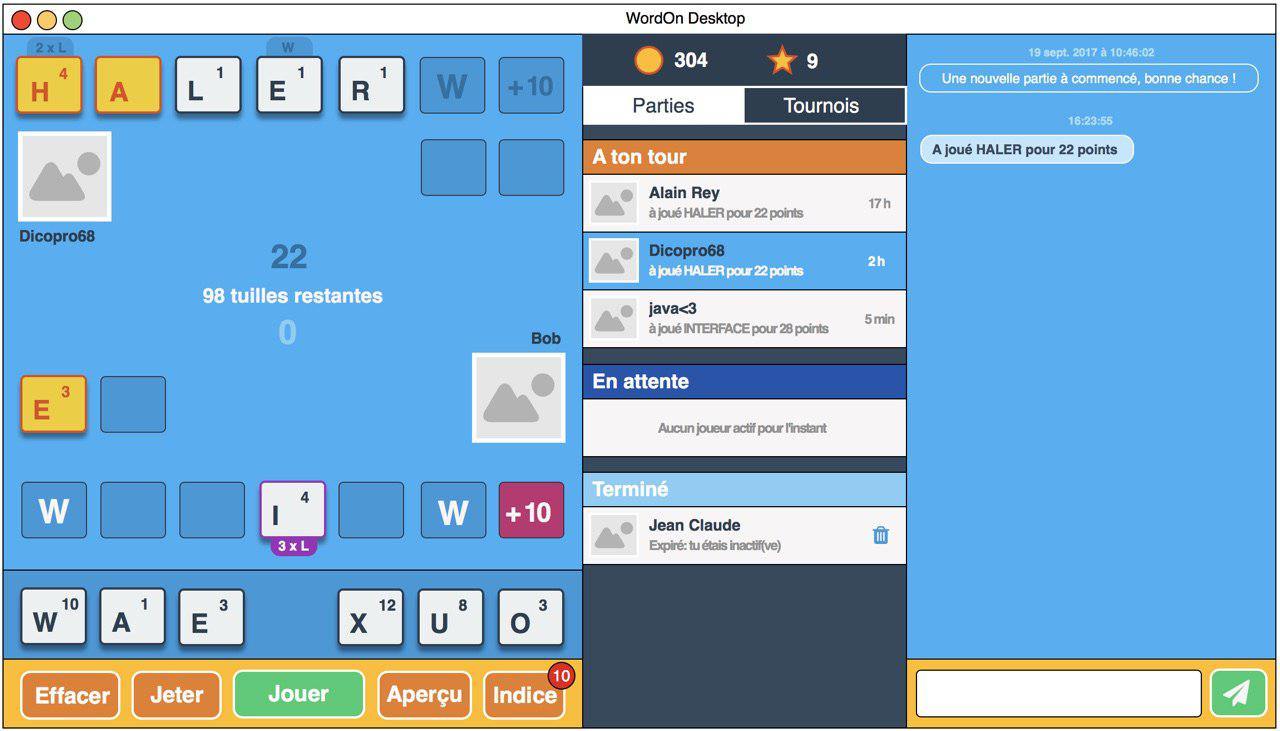
\includegraphics[width=0.6\linewidth]{img/main.jpg}
			\caption{Interface principale}
		\end{figure}
		
	\subsection{Conception}
	
	\subsection{Implémentation}
		\subsubsection{Dictionnaire / Stack}
		Nous avons effectué du reverse engineering\footnote{\textbf{Reverse engineering} :  \href{https://fr.wikipedia.org/wiki/R\%C3\%A9tro-ing\%C3\%A9nierie}{Définition Wikipédia}} afin de comprendre le fonctionnement internet du jeu.\\
		Après avoir enregistré plusieurs fois les lettres sorties par l'application mobile, nous avons pu constater et mettre en avant que le dictionnaire (les lettres tirées) sont définie par rapport à stack prédéfinit qui est simplement mélangé au début de la partie. En effet, lors d'une partie, on trouvera toujours le même nombre de fois le \textit{E} qui sort par exemple.
		
		Nous sommes arrivé au dictionnaire suivante : 
		
		\begin{table}[h]
			\centering
			\begin{tabular}{cc}
				\textbf{Lettre} & \textbf{Nombre} \\
				A     & 12 \\
				B     & 2 \\
				C     & 3 \\
				D     & 3 \\
				E     & 17 \\
				F     & 2 \\
				G     & 2 \\
				H     & 2 \\
				I     & 10 \\
				J     & 1 \\
				K     & 1 \\
				L     & 5 \\
				M     & 3 \\
				N     & 6 \\
				O     & 7 \\
				P     & 3 \\
				Q     & 1 \\
				R     & 7 \\
				S     & 8 \\
				T     & 6 \\
				U     & 8 \\
				V     & 1 \\
				W     & 1 \\
				X     & 1 \\
				Y     & 1 \\
				Z     & 1 \\
				\textit{JOKER} & 2 
			\end{tabular}
			\caption{Nombre d'occurence de chaque lettre dans notre dictionnaire}
		\end{table}
		
		\subsubsection{Algorithme tirage aléatoire}
		Suite à la mise en avant du dictionnaire, soit du stack définit de lettre qui peuvent sortir au cours d'une partie, nous avons analysé leur ordre de sortie en essayant de mettre un avant un paterne, ou toutes autres logique. \\
		Nous avons constaté que l'ordre d'arrivée des lettres est purement aléatoire malgré les apparences. En effet, au fur et à mesure que l'on avance dans une partie, on va acumuler des lettres peut utilisées de la langue française, telle que le \textit{J}, \textit{K}, \textit{V}, \textit{W}, \textit{X}, etc, ce qui rend un apparence seulement, la partie plus dur lorsque nous arrivons au terme.
		
		\subsubsection{Communication}
	
	\subsection{Tests}
	\subsubsection{Bug connu}
	
	\subsubsection{Fonctionnalité pouvant être ajoutée}
	
	\section{Technologie utilisée}
	Nous avons décidé de coder et développer notre application sans framework. En effet, aucun des frameworks connus ne nous aurait réellement aidés par rapport à nos beosin. De plus, prendre du temps pour comprendre et savoir utiliser correctement un ou plusieurs nouveaux frameworks aurait pû nous prendre beaucoup de temps. \\
	C'est pour ces raisons que nous choisis de coder principalement notre projet en pure Java, y compris pour toute la partie communication. 
	
		\subsection{JUnit}
		JUnit est un framework Java permettant de faire des tests unitaires. Ce dernier comporte de nombreuses méthodes afin d'automatiser les tests, et est utilisé par \hyperref[maven]{Maven}.\\
		Il permet par exemple de comparer des valeurs attendues de méthode avec ce que l'on reçoit vraiment. On peut tester l'intégralité des communications avec un tel système. De plus, il permet de s'assurer que même lors du développement d'un tel projet, les méthodes et fonctions codées précédemment n'ont pas un comportement différent en fonction du contexte d'appel. 
		
		\subsection{JavaFX}
		JavaFX est une bibliothèque d'interface graphique. Nous l'avons utilisée, avec l'aide de SceneBuilder\footnote{\textbf{SceneBuilder} : \href{http://gluonhq.com/products/scene-builder/}{gluonhq.com/products/scene-builder/}} qui permet de créer des interfaces graphiques de manière intuitive et visuelle. \\
		Cette librairie permet également de gérer tout ce qui est des interactions avec notre environnement graphique à l'aide de \textit{listener} qu'on peut lier à nos briques, nos éléments graphiques. 
		
		\subsection{GitHub}
		GitHub\footnote{\textbf{GitGub} : \href{http:/github.com}{github.com}} utilise la technologie git qui permet de gérer les fichiers d'un projet sur différentes branches, tout en faisant du versionning en ligne. Il offre également la possibilité de gérer les issues avec un système communautaire (du groupe) pour la résolution, mais également une gestion de planning et d'attribution de tâches. \\
		Ceci nous a permis de bien pouvoir séparer le travail et les parties, pour ensuite, une fois validé par les tests, les intégrer dans notre projet, soit sur la branche master. 
		
		\subsection{Apache Maven} \label{maven}
		Maven est un outil de gestion et d'automatisation de projet Java. Il permet notamment d'automatiser les dépendances de notre projet en téléchargent automatiquement les librairies utilisées par les autres membres du groupe. Il permet également de tester le projet en lançant tout les tests de notre projet avant de le compiler afin de garantir du bon fonctionnement de ce dernier. 
		
		\subsection{Docker}
		Docker est une technologie qui tent à se répendre de plus en plus. Ce dernier permet de lancer des machines virtuelles dans des containers tout en automatisant le déploiement de ces derniers. 
		
		Pour ce projet nous avons réaliser un petit script qui permet de compiler notre projet avec Maven tout en verifiant qu'il passe tout nos test JUnit, puis il va lancer (et télécharger au besoin) un serveur MySQL pour notre base de données, mais également un serveur PhpMyAdmin pour l'administration de la base de données, et pour finir une machine virtuel linux qui va inplémenter et lancer le serveur Java de notre application. 
	
	\section{Conclusion}
	
	\newpage
	\section{Annexes}

	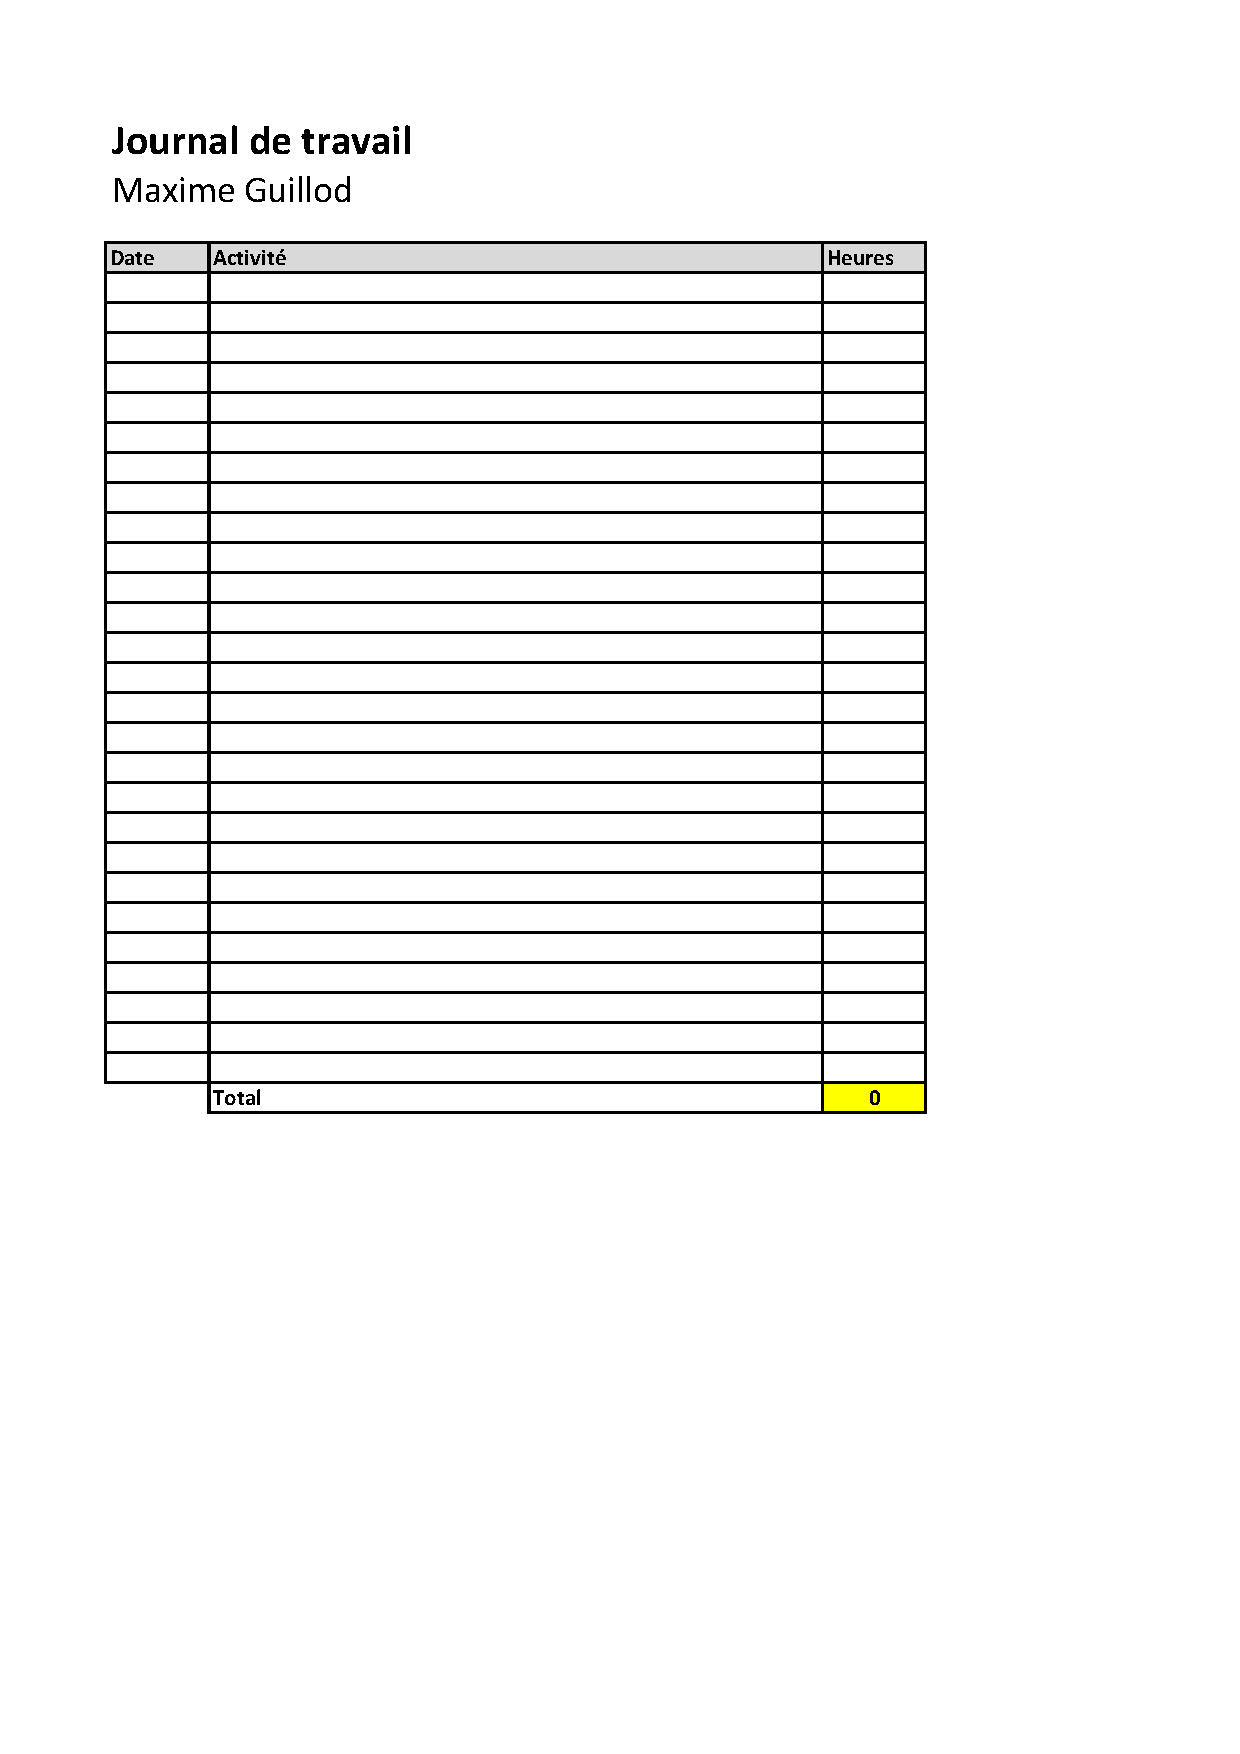
\includepdf[scale=0.95, pagecommand={}]{journalTravail/vide.pdf}
	%\includepdf[scale=0.95, pagecommand={}]{journalTravail/Lawrence.pdf}
	%\includepdf[scale=0.95, pagecommand={}]{journalTravail/Miguel.pdf}
	%\includepdf[scale=0.95, pagecommand={}]{journalTravail/Cotza.pdf}
	%\includepdf[scale=0.95, pagecommand={}]{journalTravail/Jimmy.pdf}
	%\includepdf[scale=0.95, pagecommand={}]{journalTravail/Tony.pdf}
	%\includepdf[scale=0.95, pagecommand={}]{journalTravail/Maxime.pdf}
	
	
	
\end{document}

